\section{Resoconto attività di verifica}
In questa sezione sono descritte le attività di verifica svolte sui documenti che vengono presentati alle revisioni di avanzamento. Qualora una verifica riscontrasse un problema su un documento, nella sezione \S B si discuterà di quali siano i possibili miglioramenti.
Inoltre verranno utlizzate delle sigle per fare riferimento al periodo in cui sono stati rilevati i risultati delle verifiche. Le sigle sono le seguenti:
\begin{itemize}
\item \textbf{An}: Analisi;
\item \textbf{TB}: Technology Baseline;
\item \textbf{PB}: Product Baseline;
\item \textbf{VC}: Validazione e Collaudo. 
\end{itemize}

\subsection{Analisi dei documenti}
\subsubsection{Analisi statica}
L'analisi dei documenti mediante Walkthrough (vedi \textit{Norme di Progetto}) ha portato all'individuazione di alcuni errori frequenti a partire dai quali è stata stilata una check list. In questo modo sarà possibile applicare l’Inspection (vedi \textit{Norme di Progetto}) per le future attività di verifica.


\paragraph{Esiti Indice di Gulpease} \mbox{} \\
\begin{longtable}{c c c c c c}
\rowcolor{white}\caption{Esiti verifica documenti con Indice di Gulpease} \\
		\rowcolor{redafk}
\textcolor{white}{\textbf{Documento}} &
\textcolor{white}{\textbf{An}} &
\textcolor{white}{\textbf{TB}} &
\textcolor{white}{\textbf{PB}} &
\textcolor{white}{\textbf{VC}} &
\textcolor{white}{\textbf{Esito}} \\
		\endfirsthead
		\rowcolor{white}\caption[]{(continua)} \\
		\rowcolor{redafk}
\textcolor{white}{\textbf{Documento}} &
\textcolor{white}{\textbf{An}} &
\textcolor{white}{\textbf{TB}} &
\textcolor{white}{\textbf{PB}} &
\textcolor{white}{\textbf{VC}} &
\textcolor{white}{\textbf{Esito}} \\
		\endhead
		\textit{Analisi dei Requisiti} & 70 & 73 & - & - & Ottimale \\
		\textit{Glossario} & 74 & 74 & - & - & Ottimale \\
		\textit{Norme di Progetto} & 67 & 69 & - & - & Ottimale \\
		\textit{Piano di Progetto} & 69 & 71 & - & - & Ottimale \\
		\textit{Piano di Qualifica} & 72 & 71 & - & - & Ottimale \\
		\textit{Studio di Fattibilità} & 70 & - & - & - & Ottimale \\
		\textit{Media Verbali} & 71 & 74 & - & - & Ottimale\\
\end{longtable}

\begin{figure}[H]
\centering
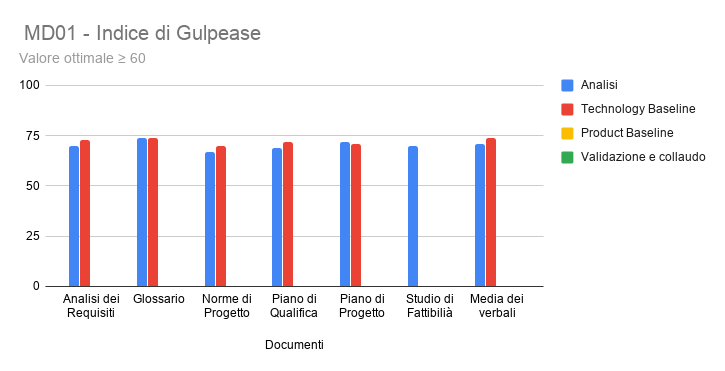
\includegraphics[scale=0.5]{./img/MD01_gulpease.png}
\caption{Grafico relativo ai dati di MD01 - Indice di Gulpease}
\end{figure}

\paragraph{Esiti Indice Fog} \mbox{} \\
\begin{longtable}{c c c c c c}
\rowcolor{white}\caption{Tabella Indice Fog} \\
		\rowcolor{redafk}
\textcolor{white}{\textbf{Attività}} &
\textcolor{white}{\textbf{An}} &
\textcolor{white}{\textbf{TB}} &
\textcolor{white}{\textbf{PB}} &
\textcolor{white}{\textbf{VC}} &
\textcolor{white}{\textbf{Riscontro}}  \\
		\endfirsthead
		\rowcolor{white}\caption[]{(continua)} \\
		\rowcolor{redafk}
\textcolor{white}{\textbf{Attività}} &
\textcolor{white}{\textbf{An}} &
\textcolor{white}{\textbf{TB}} &
\textcolor{white}{\textbf{PB}} &
\textcolor{white}{\textbf{VC}} &
\textcolor{white}{\textbf{Riscontro}}  \\
		\endhead
\textit{Analisi dei Requisiti} & 18 & 17 & - & - & Accettabile\\
\textit{Glossario} & 15 & 15 & - & - & Accettabile \\
\textit{Norme di Progetto} & 20 & 18 & - & - & Accettabile\\
\textit{Piano di Progetto} & 18 & 20 & - & - & Accettabile\\
\textit{Piano di Qualifica} & 20 & 20 & - & - & Accettabile\\
\textit{Studio di Fattibilità} & 14 & - & & & Accettabile\\
\textit{Media Verbali} & 8 & 6 & - & - & Ottimale\\
\end{longtable}

\begin{figure}[H]
\centering
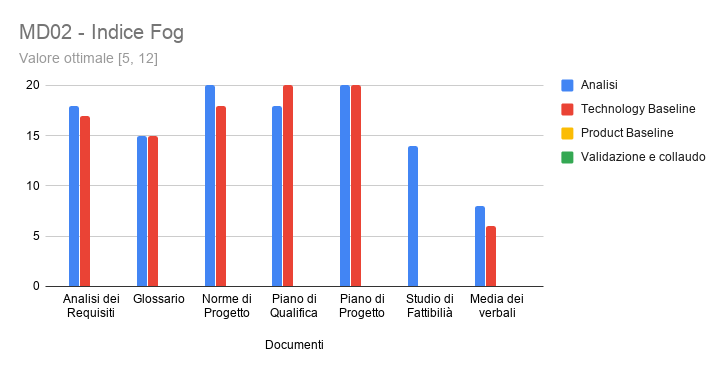
\includegraphics[scale=0.5]{./img/MD02_fog.png}
\caption{Grafico relativo ai dati di MD02 - Indice Fog}
\end{figure}

\subsection{Analisi dei processi}
\subsubsection{Esiti MP01 - Schedule Variance} 
\begin{longtable}{c c c c c c}
\rowcolor{white}\caption{Esiti verifica Schedule Variance} \\
		\rowcolor{redafk}
\textcolor{white}{\textbf{Attività}} &
\textcolor{white}{\textbf{An}} &
\textcolor{white}{\textbf{TB}} &
\textcolor{white}{\textbf{PB}} &
\textcolor{white}{\textbf{VC}} &
\textcolor{white}{\textbf{Riscontro}} \\
		\endfirsthead
		\rowcolor{white}\caption[]{(continua)} \\
		\rowcolor{redafk}
\textcolor{white}{\textbf{Attività}} &
\textcolor{white}{\textbf{An}} &
\textcolor{white}{\textbf{TB}} &
\textcolor{white}{\textbf{PB}} &
\textcolor{white}{\textbf{VC}} &
\textcolor{white}{\textbf{Riscontro}} \\
		\endhead
\textit{Analisi dei Requisiti} & 
1 &
1 &
- &
- &
Accettabile \\
\textit{Glossario} & 
0 &
0 &
- &
- &
Ottimale \\
\textit{Norme di Progetto} & 
0 &
1 &
- &
- &
Accettabile \\
\textit{Piano di Qualifica} & 
1 &
-2 &
- &
- &
Ottimale \\
\textit{Piano di Progetto} & 
1 &
0 &
- &
- &
Ottimale \\
\textit{Studio di Fattibilià} & 
0 &
- &
- &
- &
Ottimale \\
\end{longtable}

\begin{figure}[H]
\centering
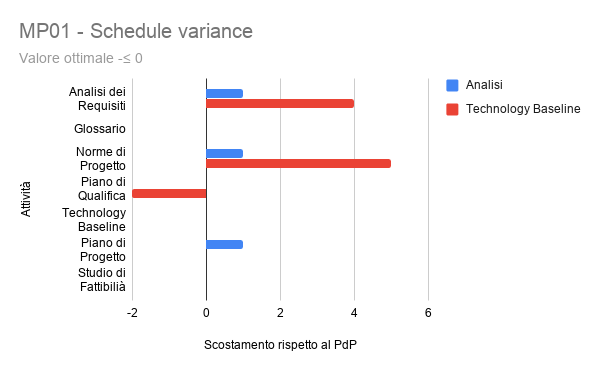
\includegraphics[scale=0.6]{./img/MP01_schedule_variance.png}
\caption{Grafico relativo ai dati di MP01 - Schedule Variance}
\end{figure}

\subsubsection{Esiti MP02 - Budget Variance}
\begin{longtable}{c c c c c}
\rowcolor{white}\caption{Esiti Budget Variance} \\
		\rowcolor{redafk}
\textcolor{white}{\textbf{An}} &
\textcolor{white}{\textbf{TB}} &
\textcolor{white}{\textbf{PB}} &
\textcolor{white}{\textbf{VC}} &
\textcolor{white}{\textbf{Riscontro}} \\
-8,66$\%$ &
-1,19$\%$ &
- &
- &
Accettabile \\
\end{longtable}

\begin{figure}[H]
\centering
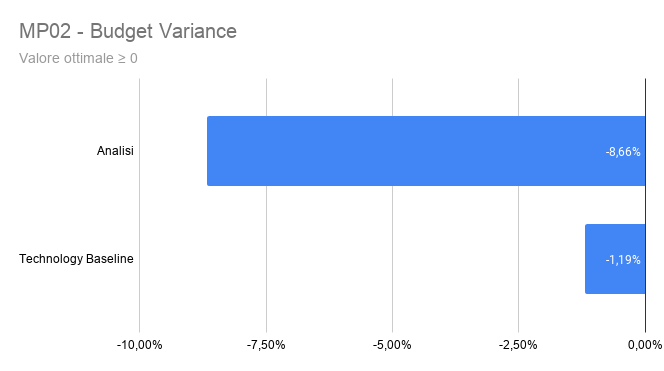
\includegraphics[scale=0.5]{./img/MP02_budget_variance.png}
\caption{Grafico relativo ai dati di MP02 - Budget Variance}
\end{figure}

\subsubsection{Esiti MP03 - Produttività} 
\begin{longtable}{c c c c c c}
\rowcolor{white}\caption{Esiti della Produttività} \\
		\rowcolor{redafk}
\textcolor{white}{\textbf{Membro}} &
\textcolor{white}{\textbf{An}} &
\textcolor{white}{\textbf{TB}} &
\textcolor{white}{\textbf{PB}} &
\textcolor{white}{\textbf{VC}} &
\textcolor{white}{\textbf{Riscontro}} \\
		\endfirsthead
		\rowcolor{white}\caption[]{(continua)} \\
		\rowcolor{redafk}
		\textcolor{white}{\textbf{Membro}} &
\textcolor{white}{\textbf{An}} &
\textcolor{white}{\textbf{TB}} &
\textcolor{white}{\textbf{PB}} &
\textcolor{white}{\textbf{VC}} &
\textcolor{white}{\textbf{Riscontro}} \\
		\endhead
Simone Federico Bergamin & 0 & 78 & - & - & Accettabile\\
Alessandro Canesso & 0 & 139 & - & - & Ottimale \\
Victor Dutca & 0 & 108 & - & - & Ottimale \\
Fouad Farid & 0 & 109 & - & - & Ottimale \\
Simone Meneghin & 0 & 93 & - & - & Accettabile\\
Olivier Utshudi & 0 & 93 & - & - & Accettabile\\
Davide Zilio & 0 & 93 & - & - & Accettabile
\end{longtable}

\begin{figure}[H]
\centering
\includegraphics[scale=0.5]{./img/MP03_produttività.png}
\caption{Grafico relativo ai dati di MP03 - Produttività}
\end{figure}

\subsection{Analisi metriche dei test}
\subsubsection{Esiti test implementati}
\begin{longtable}{c c}
\rowcolor{white}\caption{Esiti dei test implementati} \\
	\rowcolor{redafk}
\textcolor{white}{\textbf{Codice test}} &
\textcolor{white}{\textbf{Esito}} \\
	\endfirsthead
		\rowcolor{white}\caption[]{(continua)} \\
		\rowcolor{redafk}
\textcolor{white}{\textbf{Codice test}} &
\textcolor{white}{\textbf{Esito}} \\
	\endhead
	TSOF1 & Passato \\
	TSOF1.1 & Passato \\ 
	TSOF1.2 & Passato \\
	TSOF1.3 & Passato \\
	TSOF1.3.1 & Passato \\
	TSOF1.3.2 & Passato \\
	TSOF1.4 & Passato \\
	TSOF2 & Passato \\
	TSOF2.1 & Passato \\
	TSOF2.2 & Passato  \\
	TSOF3.2 & Passato 
	
\end{longtable}

\subsubsection{Esiti MS08/MS09 - Passed/Failed Test Case Percentage}
\begin{longtable}{c c c}
\rowcolor{white}\caption{Esiti PTCP-FTCP} \\
	\rowcolor{redafk}
\textcolor{white}{\textbf{Metrica}} &
\textcolor{white}{\textbf{Percentuale}} & 
\textcolor{white}{\textbf{Riscontro}} \\
	\endfirsthead
\textcolor{white}{\textbf{Metrica}} &
\textcolor{white}{\textbf{Percentuale}} & 
\textcolor{white}{\textbf{Riscontro}} \\
	\endhead
	PTCP & 100\% & Ottimale\\
	FTCP & 0\% & Ottimale\\
\end{longtable}

\begin{figure}[H]
\centering
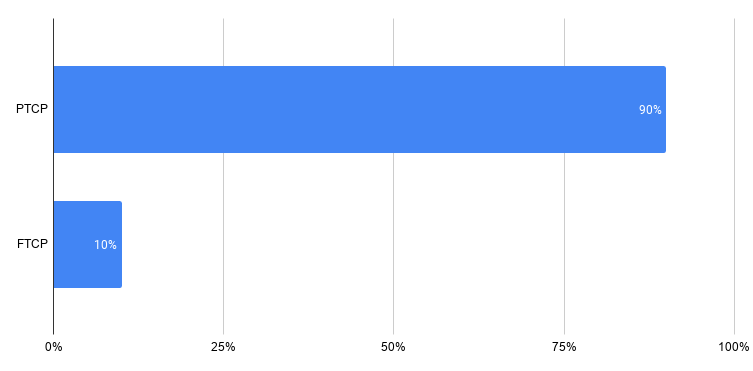
\includegraphics[scale=0.5]{./img/MS08-MS09.png}
\caption{Grafico relativo ai dati di MS08-MS09 PTCP-FTCP}
\end{figure}

\pagebreak
\subsection{Analisi metriche del software}
\subsubsection{Esiti MS04 - Commenti per Linee di Codice}
\begin{longtable}{c c c c}
\rowcolor{white}\caption{Esiti MS04} \\
	\rowcolor{redafk}
	\textcolor{white}{\textbf{Tot\_LOC}} &
	\textcolor{white}{\textbf{Tot\_commenti}} &
\textcolor{white}{\textbf{Rapporto}} &
\textcolor{white}{\textbf{Esito}} \\
	\endfirsthead
		\rowcolor{white}\caption[]{(continua)} \\
		\rowcolor{redafk}
		\textcolor{white}{\textbf{Tot\_LOC}} &
\textcolor{white}{\textbf{Tot\_commenti}} &
\textcolor{white}{\textbf{Rapporto}} & 
\textcolor{white}{\textbf{Esito}} \\
	\endhead
	713 & 7 & 0.01 & Non accettabile\\	
\end{longtable}

\begin{figure}[H]
\centering
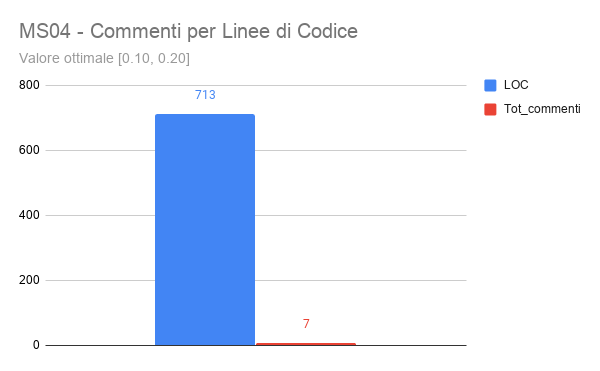
\includegraphics[scale=0.40]{./img/MS04.png}
\caption{Grafico relativo ai dati di MS04 - Commenti per LOC}
\end{figure}

\subsubsection{Esiti MS05-MS06 - Fan In/Fan Out}
\begin{longtable}{c c}
\rowcolor{white}\caption{Esiti MS05-MS06} \\
	\rowcolor{redafk}
	\textcolor{white}{\textbf{Fan In}} &
	\textcolor{white}{\textbf{Fan Out}}\\
	\endfirsthead
		\rowcolor{white}\caption[]{(continua)} \\
		\rowcolor{redafk}
	\textcolor{white}{\textbf{Fan In}} &
	\textcolor{white}{\textbf{Fan Out}}\\
	\endhead
	31 & 26\\	
\end{longtable}

\begin{figure}[H]
\centering
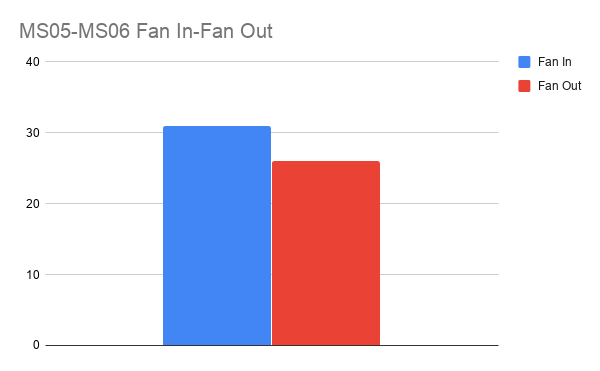
\includegraphics[scale=0.45]{./img/MS05-MS06.png}
\caption{Grafico relativo ai dati di MS05-MS06 - Fan In/Fan Out}
\end{figure}




\begin{comment}
\begin{longtable}{C{2cm} C{1.2cm} C{3cm} C{1.5cm} C{1.5cm} C{1.5cm} C{1.5cm} C{1.5cm}}
\rowcolor{white}\caption{Esiti PTCP-FTCP} \\
	\rowcolor{redafk}
\textcolor{white}{\textbf{Classe}} &
\textcolor{white}{\textbf{MS02}} &
\textcolor{white}{\textbf{Metodo}} &
\textcolor{white}{\textbf{MS01}} &
\textcolor{white}{\textbf{MS03}} & 
\textcolor{white}{\textbf{MS04}} & 
\textcolor{white}{\textbf{MS05}} & 
\textcolor{white}{\textbf{MS06}} \\
	\endfirsthead
		\rowcolor{white}\caption[]{(continua)} \\
		\rowcolor{redafk}
\textcolor{white}{\textbf{Classe}} &
\textcolor{white}{\textbf{MS02}} &
\textcolor{white}{\textbf{Metodo}} &
\textcolor{white}{\textbf{MS01}} &
\textcolor{white}{\textbf{MS03}} & 
\textcolor{white}{\textbf{MS04}} & 
\textcolor{white}{\textbf{MS05}} & 
\textcolor{white}{\textbf{MS06}} \\
	\endhead
	header.jsx & 1 & render() & 6 & 0 & 0 & 0 & 1 \\
	state\_controller.jsx & 4 & changeValue() \newline 
								errorAlg() \newline
								handleForce() \newline
								render() &	1 \newline 1 \newline 1 \newline 12 &
								1 \newline 1 \newline 2 \newline 0 &
								0 \newline 0 \newline 0 \newline 0 &
								1 \newline 1 \newline 1 \newline 3 &
								0 \newline 0 \newline 0 \newline 0 \\
\end{longtable}
\end{comment}